

\PassOptionsToPackage{dvipsnames}{xcolor}
\documentclass[aspectratio=169,11pt]{beamer}

% ===== CONFIGURATION (edit these) ====================================
\newcommand{\teamname}{The Three Musketeers}
\newcommand{\topicchoice}{Topic 3 -- AI News Briefing Service}
\newcommand{\memberone}{Ali Huseynli}
\newcommand{\membertwo}{Alish Hajiyev}
\newcommand{\memberthree}{Elsen Samadzada}
\newcommand{\repolink}{https://github.com/aliasefoglu/Final_Project_01.git}

\newcommand{\coursecode}{AI-ENG-110}
\newcommand{\coursename}{Software Engineering}
\newcommand{\institution}{AI Academy, National AI Center}
\newcommand{\semester}{Spring 2026}

% ===== PACKAGES ======================================================
\usepackage[T1]{fontenc}
\usepackage[utf8]{inputenc}
\usepackage{xcolor}
\usepackage{tabularx}
\usepackage{booktabs}
\usepackage{listings}
\usepackage{tikz}
\usetikzlibrary{shapes.geometric,arrows.meta,positioning,fit,backgrounds}

% ===== EARLY MACROS ==================================================
\definecolor{accent2}{HTML}{8B0000}
\newcommand{\TODO}[1]{\textcolor{accent2}{\textbf{[TODO: #1]}}}

% ===== BEAMER THEME (custom, no flashy decorations) =================
\usetheme{default}
\usefonttheme{professionalfonts}
\setbeamertemplate{navigation symbols}{}

\definecolor{accent}{HTML}{0B3D91}
\definecolor{soft}{HTML}{F2F4F8}
\definecolor{ok}{HTML}{166534}

\setbeamercolor{title}{fg=accent}
\setbeamercolor{frametitle}{fg=accent}
\setbeamercolor{section in head/foot}{bg=accent,fg=white}
\setbeamercolor{itemize item}{fg=accent}
\setbeamercolor{itemize subitem}{fg=accent}
\setbeamercolor{enumerate item}{fg=accent}
\setbeamercolor{block title}{bg=accent,fg=white}
\setbeamercolor{block body}{bg=soft,fg=black}

\setbeamerfont{title}{size=\Large,series=\bfseries}
\setbeamerfont{frametitle}{size=\large,series=\bfseries}
\setbeamerfont{footline}{size=\tiny}

% Footer with team + slide number
\setbeamertemplate{footline}{%
  \leavevmode%
  \hbox{\hspace*{2ex}\tiny\textit{\teamname{} -- \topicchoice}\hfill%
  \tiny\textit{\coursecode{} -- \semester{}}\hfill%
  \tiny\insertframenumber/\inserttotalframenumber\hspace*{2ex}}%
  \vskip1pt%
}

% ===== CODE LISTINGS =================================================
\definecolor{codegreen}{rgb}{0,0.55,0}
\definecolor{codepurple}{rgb}{0.55,0,0.78}
\lstdefinestyle{python}{
  language=Python,
  backgroundcolor=\color{soft},
  commentstyle=\color{codegreen},
  keywordstyle=\color{accent},
  stringstyle=\color{codepurple},
  basicstyle=\ttfamily\scriptsize,
  breaklines=true,
  frame=single,
  framerule=0.4pt,
  rulecolor=\color{black!30},
}

% =====================================================================
\begin{document}

% ========== SLIDE 1: TITLE ===========================================
{%
\setbeamertemplate{footline}{}
\begin{frame}[plain]
  \begin{center}
    \vspace{0.6cm}
    {\small \textsc{\institution}}\\[0.2em]
    {\small \textsc{\coursecode{} -- \coursename{} -- \semester{}}}\\[1.2em]
    \rule{0.7\textwidth}{0.6pt}\\[0.4em]
    {\Huge\bfseries\color{accent} \topicchoice}\\[0.4em]
    \rule{0.7\textwidth}{0.6pt}\\[1.2em]
    {\large \teamname}\\[0.6em]
    {\normalsize \memberone\quad\textbullet\quad\membertwo\quad\textbullet\quad\memberthree}\\[1cm]
    {\footnotesize\itshape Final Project Defense -- September 20, 2026}\\[0.4em]
    {\footnotesize\texttt{\repolink}}
  \end{center}
\end{frame}
}

% ========== SLIDE 2: PROBLEM =========================================
\begin{frame}{The problem in one sentence}
  \begin{block}{What the system does}
    A user sets topic preferences once; every day, we fetch from 6 sources, remove duplicate coverage of the same story, and hand back one personalized Markdown digest with a 2--3 sentence summary and topic/sentiment label per article.
  \end{block}

  \vspace{0.3em}
  \begin{columns}[T,onlytextwidth]
  \column{0.48\textwidth}
  \textbf{Inputs}
  \begin{itemize}
    \item 5 RSS feeds + 1 scraped HTML source
    \item A user's preferred topics \& excluded sources
  \end{itemize}

  \column{0.48\textwidth}
  \textbf{Outputs}
  \begin{itemize}
    \item \texttt{digests/YYYY-MM-DD-<user>.md}
    \item A row per article in PostgreSQL (dedup cache)
  \end{itemize}
  \end{columns}

  \vspace{0.4em}
  \textbf{Entry points:} \texttt{python -m src.cli run-daily --user <name>}, plus a bonus FastAPI web UI (signup/login/preferences) not required for Topic 3.
\end{frame}

% ========== SLIDE 3: ARCHITECTURE ====================================
\begin{frame}{Architecture}
  \textbf{Module map.} The boundary between the \emph{provided} \texttt{ai/} package and \emph{our} SE layer is shown explicitly.

  \vspace{0.3em}
  \begin{center}
  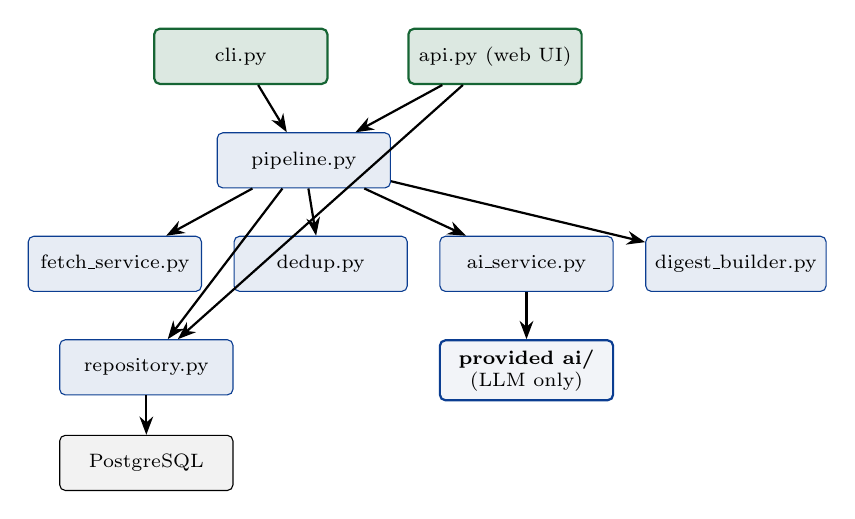
\begin{tikzpicture}[
    node distance=3mm,
    box/.style={draw,rounded corners=2pt,minimum width=2.2cm,minimum height=0.7cm,align=center,font=\scriptsize},
    aibox/.style={box,fill=soft,draw=accent,thick},
    sebox/.style={box,fill=accent!10,draw=accent},
    entry/.style={box,fill=ok!15,draw=ok,thick},
    arrow/.style={-Stealth,thick}
  ]
    \node[entry] (cli) {cli.py};
    \node[entry,right=10mm of cli] (api) {api.py (web UI)};

    \node[sebox,below=6mm of cli,xshift=8mm] (pipe) {pipeline.py};

    \node[sebox,below=6mm of pipe,xshift=-24mm] (fetch) {fetch\_service.py};
    \node[sebox,right=4mm of fetch] (dedup) {dedup.py};
    \node[sebox,right=4mm of dedup] (aisvc) {ai\_service.py};
    \node[sebox,right=4mm of aisvc] (digest) {digest\_builder.py};

    \node[aibox,below=6mm of aisvc] (ai) {\textbf{provided ai/}\\(LLM only)};
    \node[sebox,below=6mm of fetch,xshift=4mm] (repo) {repository.py};
    \node[box,below=5mm of repo,fill=gray!10] (pg) {PostgreSQL};

    \draw[arrow] (cli) -- (pipe);
    \draw[arrow] (api) -- (pipe);
    \draw[arrow] (pipe) -- (fetch);
    \draw[arrow] (pipe) -- (dedup);
    \draw[arrow] (pipe) -- (aisvc);
    \draw[arrow] (pipe) -- (digest);
    \draw[arrow] (aisvc) -- (ai);
    \draw[arrow] (pipe) -- (repo);
    \draw[arrow] (api) -- (repo);
    \draw[arrow] (repo) -- (pg);
  \end{tikzpicture}
  \end{center}

  \vspace{0.3em}
  
\end{frame}

% ========== SLIDE 4: KEY DESIGN DECISIONS ============================
\begin{frame}{Three design decisions we can defend}
  \begin{enumerate}\setlength\itemsep{0.6em}
    \item \textbf{asyncio + Semaphore over threads for fetching}\\
      Every bottleneck is I/O-bound (network waits), so asyncio's structured concurrency (gather + per-task try/except) expresses "keep going if one source fails" more directly than thread futures.
    \item \textbf{Normalized join tables over a JSONB array for preferences}\\
      Our first design stored topics as a JSONB list on \texttt{users} -- simple, but a 1NF violation. We normalized into \texttt{user\_preferred\_topics}/\texttt{user\_excluded\_sources} with a composite primary key, wrapped in one transaction for atomicity.
    \item \textbf{One retry policy per external boundary, not a shared one}\\
      \texttt{fetch\_service} and \texttt{ai\_service} each get their own \texttt{tenacity} policy (different exceptions, different backoff windows) rather than one generic retry wrapper, since a fetch timeout and an LLM provider error need different handling.
  \end{enumerate}

  \vspace{0.6em}
\end{frame}

% ========== SLIDE 5: CONCURRENCY (THE BENCHMARK) =====================
\begin{frame}{Concurrency: the benchmark}
  \textbf{Workload:} \texttt{scripts/bench.py --N 20} -- 20 fetch operations cycling the 6 configured sources

  \vspace{0.4em}
  \begin{center}\small
  \begin{tabular}{lcc}
    \toprule
    & \textbf{Sequential (sem=1)} & \textbf{Concurrent (sem=8)} \\
    \midrule
    Wall-clock (s) & 13.79 & 3.00 \\
    Speedup        & 1.0$\times$ & \textbf{4.6$\times$} \\
    \bottomrule
  \end{tabular}
  \end{center}

  \vspace{0.4em}
  \textbf{Bottleneck named:} per-source network RTT, plus the Reuters scrape source failing (401 Forbidden, see next slide) and retrying 3$\times$ on every single one of the 20 operations -- fixed overhead concurrency can't remove.\\
  \textbf{Command:} \texttt{docker compose run --rm app python scripts/bench.py --N 20}
\end{frame}

% ========== SLIDE 6: ROBUSTNESS STORY ================================
\begin{frame}{Robustness: one concrete failure mode}
  \textbf{Scenario (real, not staged):} our Reuters HTML-scrape source returned \texttt{401 Forbidden} on \emph{every} request during our real benchmark run -- Reuters blocks scripted requests.

  \vspace{0.3em}
  \textbf{How we found it:} not a planned chaos test -- it surfaced on its own while running \texttt{scripts/bench.py --N 20} against the real internet.

  \vspace{0.3em}
  \textbf{What the system did:}
  \begin{itemize}\setlength\itemsep{0.3em}
    \item Retry: tenacity retried 3$\times$ with exponential backoff on every single attempt -- and still failed every time.
    \item Isolate: \texttt{fetch\_all\_sources} caught it per-source; the other 5 RSS sources were unaffected.
    \item Log: \texttt{"Source ... failed after retries; continuing without it."} -- full traceback preserved.
    \item Degrade: the benchmark still completed and reported a valid 4.6$\times$ speedup using only the succeeding sources.
  \end{itemize}
  
\end{frame}

% ========== SLIDE 7: DEMO ============================================
\begin{frame}[fragile]{Live demo (or scripted demo)}
  \begin{block}{What we will run}
    The full pipeline for one user, live: fetch $\to$ dedup $\to$ summarize $\to$ digest, printed straight to the terminal.
  \end{block}

  \vspace{0.4em}
  \textbf{Demo command (works inside Docker):}
  \begin{lstlisting}[style=python,language=bash,numbers=none]
$ docker compose run --rm app python scripts/demo.py --user khagani
\end{lstlisting}

  \vspace{0.4em}
  \begin{itemize}
    \item Watch the log lines: fetched-article count, dedup rate, then one LLM call per surviving article.
  \end{itemize}

  \vspace{0.3em}
\end{frame}

% ========== SLIDE 8: TESTING =========================================
\begin{frame}{Testing}
  \begin{columns}[T,onlytextwidth]
  \column{0.55\textwidth}
  \textbf{Coverage \& shape}
  \begin{itemize}\setlength\itemsep{0.3em}
    \item \texttt{src/} coverage: \textbf{86.7\%} (90\% blended w/ \texttt{ai/})
    \item Provided \texttt{ai/} smoke tests: \textcolor{ok}{\textbf{passing (15/15)}}
    \item 69 tests total: 54 ours + 15 instructor smoke tests
    \item All 69 pass \emph{inside Docker}, not just locally
  \end{itemize}

  \column{0.42\textwidth}
  \textbf{Three tests worth calling out}
  \begin{itemize}\setlength\itemsep{0.3em}
    \item \texttt{test\_run\_daily\_pipeline\_happy\_path}
    \item \texttt{test\_fetch\_all\_sources\_runs\_sources\_concurrently}
    \item \texttt{test\_run\_daily\_pipeline\_skips\_articles\_that\_fail\_ai\_labeling}
  \end{itemize}
  \end{columns}

  \vspace{0.6em}
  \begin{block}{Tooling}
    \texttt{pytest} + \texttt{pytest-asyncio} + \texttt{pytest-cov} + \texttt{respx}. \textbf{mypy: 0 errors in our code}
  \end{block}
\end{frame}

% ========== SLIDE 9: LIMITATIONS + FUTURE ============================
\begin{frame}{Limitations \& what we'd do next}
  \textbf{Where the system is brittle today}
  \begin{itemize}\setlength\itemsep{0.3em}
    \item Confirmed, not hypothetical: Reuters actively blocks our scraper (401 Forbidden, every request).
    \item No multi-provider LLM failover -- Gemini's free tier (5/min, 20/day) exhausted mid-run in testing; we cannot fail over to a second provider automatically.
  \end{itemize}

  \vspace{0.4em}
  \textbf{Given another week we would}
  \begin{enumerate}\setlength\itemsep{0.3em}
    \item Fix the preferences-form validation gap above.
    \item Add a real integration test against a live test PostgreSQL instance, not just a mocked Repository.
  \end{enumerate}
\end{frame}

% ========== SLIDE 10: TEAM CONTRIBUTIONS =============================
\begin{frame}{Team contributions}
  \begin{center}\small
  \begin{tabularx}{\linewidth}{lXl}
    \toprule
    \textbf{Member} & \textbf{Primary ownership}\\
    \midrule
    \memberone   & config, models, repository, schema, CLI, tests \\
    \membertwo   & AI service, digest builder, scheduler, web UI, Docker \\
    \memberthree & fetch service, dedup, pipeline, benchmark, UI styling \\
    \bottomrule
  \end{tabularx}
  \end{center}


  \vspace{0.4em}
  \begin{block}{We can all answer:}
    Any of us can walk through any module on demand. Pick a file --- we'll defend it.
  \end{block}

  \vspace{0.4em}
  
\end{frame}

% ========== SLIDE 11: THANK YOU / Q&A ================================
{%
\setbeamertemplate{footline}{}
\begin{frame}[plain]
  \begin{center}
    \vspace{1cm}
    {\Huge\bfseries\color{accent} Questions?}\\[1.2em]
    \rule{0.5\textwidth}{0.6pt}\\[1.2em]
    {\large \teamname}\\[0.6em]
    {\normalsize \texttt{\repolink}}\\[1cm]
    
  \end{center}
\end{frame}
}

\end{document}
